Die Kollisionsauflösung L3 \ref{l3} soll in dieser Arbeit zwar nicht explizit behandelt, bzw. nicht umgesetzt werden, jedoch ist eine kurze Evaluation zur Ermittlung der Anforderungen für L2 unumgänglich.
L3 stellt direkte Anforderungen zu Zusatzinformationen um die passenden Konsequenzen der Kollision zu ermitteln. Diese Informationen liefert der Algorithmus in L2 (oft als Nebenprodukt). Beispiele sind Ort des ersten Kontakts zweier Objekte, Zeit oder beteiligte Merkmale an der Kollision.\\

Auch in L3 gelten Überlegungen bezüglich physikalischem Realismus (vgl. \ref{sec:physical_realism}).


\begin{figure}
	\centering
	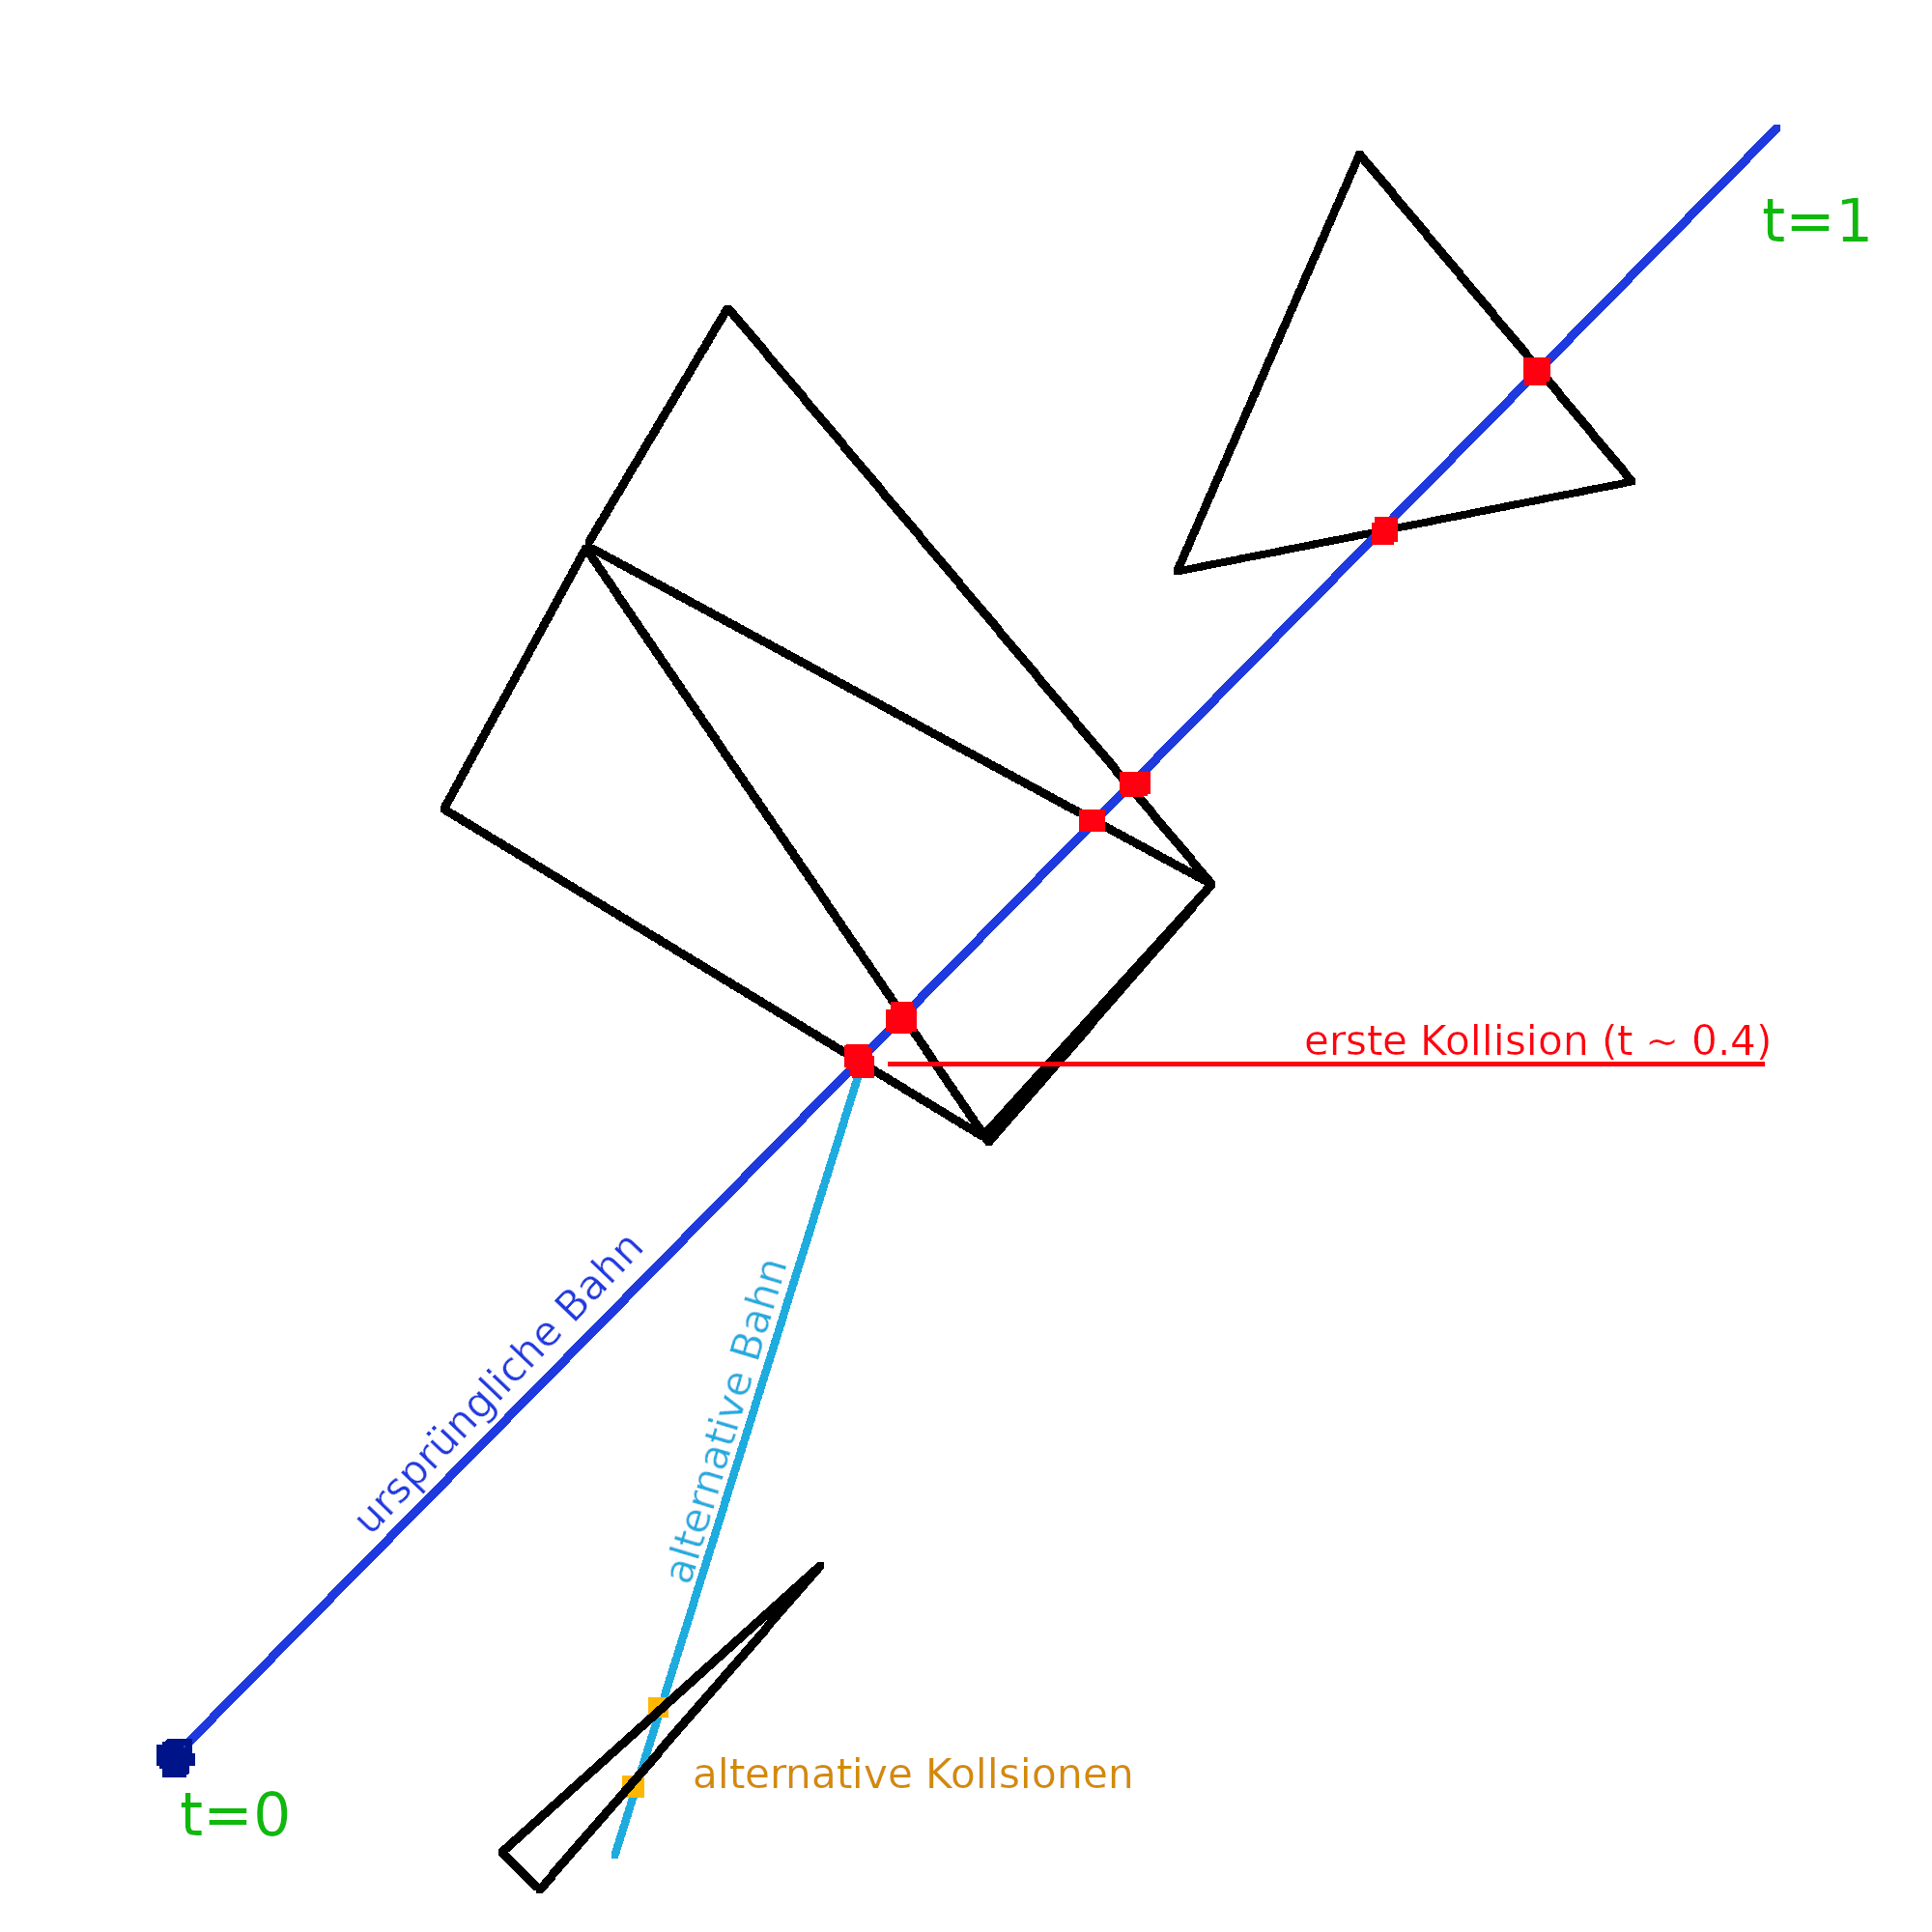
\includegraphics[width=0.6\textwidth]{./res/l3_col.png}
	\caption{2D Kollisionsszenario mit alternativen Bewegungsbahnen eines Projektils an Kollisionskörpern}
	\label{fig:l3col}
\end{figure}

Die vorhandenen Freiheitsgrade sollen im Folgenden im Beispiel verdeutlicht werden. Für die folgenden Überlegungen wird daher eine geltende Physik angenommen:
\begin{enumerate}
	\item Ein Projektil kann durch Kollision abgelenkt werden.
	\item Ein Projektil kann bei einer Kollision einen Körper durchschlagen.
\end{enumerate}

Die Abbildung~\ref{fig:l3col} zeigt mögliche Interpretationen eines Kollisionsszenario unter der postulierten Physik.
Auf der Abbildung in dunkelblau zu sehen ist die ursprüngliche Bahn des Projektils, welche innerhalb eines Ticks ($t_0$ bis $t_1$) durch zwei Körper verliefe.
Zum Zeitpunkt $t_0$ ist die in hellblau gekennzeichnete Linie der alternativen Flugbahn des Projektils noch unbekannt! Diese kann erst mit der Ermittlung der ersten Kollision errechnet werden.
Über einen L2-Algorithmus werden die rot gekennzeichneten Kollisionspunkte bekannt.\\
\\
In der L3-Schicht muss nun entschieden werden, wie mit der gegebenen Information umgegangen wird. Mehr noch: Welche Information wird tatsächlich gebraucht.\\
Es werden beispielhaft Aufösungsoptionen und Konsequenzen gelistet.
\begin{itemize}
	\item[O1] Akkurate Auflösung\\
		Konsequenzen:
		\begin{itemize}
			\item Errechnete Kollisionen nach der ersten Kollision sind ungültig. Dies gilt sowohl für L1 als auch L2! (Projektil kann abgeprallt sein oder kann durchschlagen haben, was vor der ersten Kollision noch nicht bekannt war.)\\
				$\Rightarrow$ Algorithmusanforderung: Nur die erste Kollision muss ermittelt werden.
			\item Kollisionen nach der ersten Kollision müssen neu errechnet werden (Projektil abgeprallt oder Durchschlag?, ursprünglicher oder alternativer Pfad, vgl.~Abbildung~\ref{fig:l3col})\\
				$\Rightarrow$ iterativer/rekursiver Algorithmus $\Rightarrow$ Stellt die Frage zur maximalen Iterationstiefe, da potentiell unendlich viele Iterationen, aber Begrenzung durch Tick muss eingehalten werden.
		\end{itemize}

	\item[O2] Maximal eine Kollision erlaubt pro Tick\\
		Konsequenzen:
		\begin{itemize}
			\item Kollisionsverhalten nicht realitätsgetreu (Kollisionen nach erster Kollision treten nicht auf)
			\item Festlegung: Verhalten der Kollisionspartner nach der ersten Kollision zum Zeitpunkt dieser: Verharren, weiterbewegung im nächsten Tick.
			\item Algorithmus ist konstant (im Sinne von nicht iterativ)
		\end{itemize}
	\item[O3] Zustandsänderung von Objekten nur am Ende des Ticks.\\
		Konsequenzen:
		\begin{itemize}
			\item Bei abprallendem Projektil: Kursänderung des Projektils erst bei $t_1$, alternative Kollisionen werden nicht erkannt.\\
				$\Rightarrow$ nicht realitätsgetreu
			\item Bei penetrierendem Projektil: Diskrepanz zwischen wie weit das Projektil physikalisch penetriert und der zurückgelegt weg zwischen $t_0$ und $t_1$.
				$\Rightarrow$ Schwierigkeiten in der Umsetzung des Durchschlagsverhaltens.
			\item Algorithmus ist konstant (im Sinne von nicht iterativ)
		\end{itemize}
\end{itemize}

Sind die Realitätsungetreuheiten in O2/O3 vertretbar? Wie hoch ist die Auftrittswahrscheinlichkeit in einer Konkreten Anwendung?\\
\\
Anzustreben ist O1, aber um die Tickgrenzen einzuhalten muss unter Umständen die Iterations-/Rekursionstiefe beschränkt werden. O2/O3 könnten verwendet werden um eine O1-Iteration zum vorzeitigen Abschluss zu bringen. Nötig ist die Evaluierung der Kritikalität der Diskrepanz zu O1 mit unendlicher Iterationstiefe.
 
Ein interessanter Fehler bezogen auf L3 in freier Wildbahn ist in \cite{skyrimwallglitch} zu sehen. Es handelt sich dabei um einen Glitch im Spiel The Elder Scrolls V:Skyrim. Dabei wird eine gleichzeitige Kollision des Spielermodells, eines Objekts und einer Wand oder Tür provoziert. Die Kollision, bzw. die wiederholten Kollisionen zwischen dem Spielermodell, dem Objekt (Kessel/Teller/Korb) und der Wand/Tür werden nicht richtig aufgelöst, was dazu führt, dass der Spieler durch die Wand laufen kann.


